\documentclass[a4paper,12pt]{article}
% Resize margins:
\usepackage[top=1.5cm, bottom=2cm, left=3cm, right=2cm]{geometry}
\usepackage{natbib} % Citation package to cite by name (use plainnat
% bib style).
\usepackage{graphicx} % Graphics.
\usepackage[labelformat=simple]{subcaption} % Get subfigure environment.
\renewcommand\thesubfigure{(\alph{subfigure})} % Reference subfigures in parentheses.
\usepackage{empheq} % Loads mathtools, which in turn loads amsmath.
\usepackage{amssymb, accents, bm} % Maths (accents provide tilde under symbol).
\usepackage{hyperref} % Clickable links and table of contents.
\usepackage{siunitx} % SI unit package.
\usepackage{enumerate} % Labels of the 'enumerate' environment.
\graphicspath{{img/}} % Add a path to load images.
\usepackage{pgfplots} % Plots.
\pgfplotsset{width=7cm,compat=1.12} % Set size of all plots and assure 
% compatibility backwards.
\usepackage{todonotes} % Make to-do lists and visible comments.
\usepackage{tabularx, booktabs} % Tables, Commands to getter spacing above and 
% below the various rules in the table (\toprule, \bottomrule, \midrule, and 
% \cmidrule).
\usepackage{pgfplotstable} % plot x,y data from different files.
\usepackage{pdfpages} % Include external pdf.
\newcolumntype{Y}{>{\centering\arraybackslash}X} % Center content of the table, 
% stretching column(s) with specifier X to make table as wide as specified.

% Custom underline function:
\newcommand{\ubar}[1]{\mkern 1.5mu\underline{\mkern-1.5mu#1\mkern-1.5mu}\mkern 1.5mu}
% Double underline function:
\newcommand{\uubar}[1]{\ubar{\ubar{#1}}}
% Underline bold function:
\newcommand{\ubarbold}[1]{\ubar{\bm{#1}}}
% Double underline bold function:
\newcommand{\uubarbold}[1]{\uubar{\bm{#1}}}
% Undertlilde with bold face symbol:
\newcommand{\utilde}[1]{\underaccent{\sim}{\bm{#1}}}
% Double undertlilde with bold face symbol:
\newcommand{\uutilde}[1]{\underaccent{\approx}{\bm{#1}}}

\allowdisplaybreaks

\title{Computational Nonlinear Mechanics \\ \textbf{Assignment 3:\\
    Large elasto-plastic deformations}}

\author{Rostyslav Skrypnyk\footnote{Department of Mechanics and Maritime Sciences,
    rostyslav.skrypnyk@chalmers.se}}

\date{\today}

\begin{document}

\maketitle
\tableofcontents

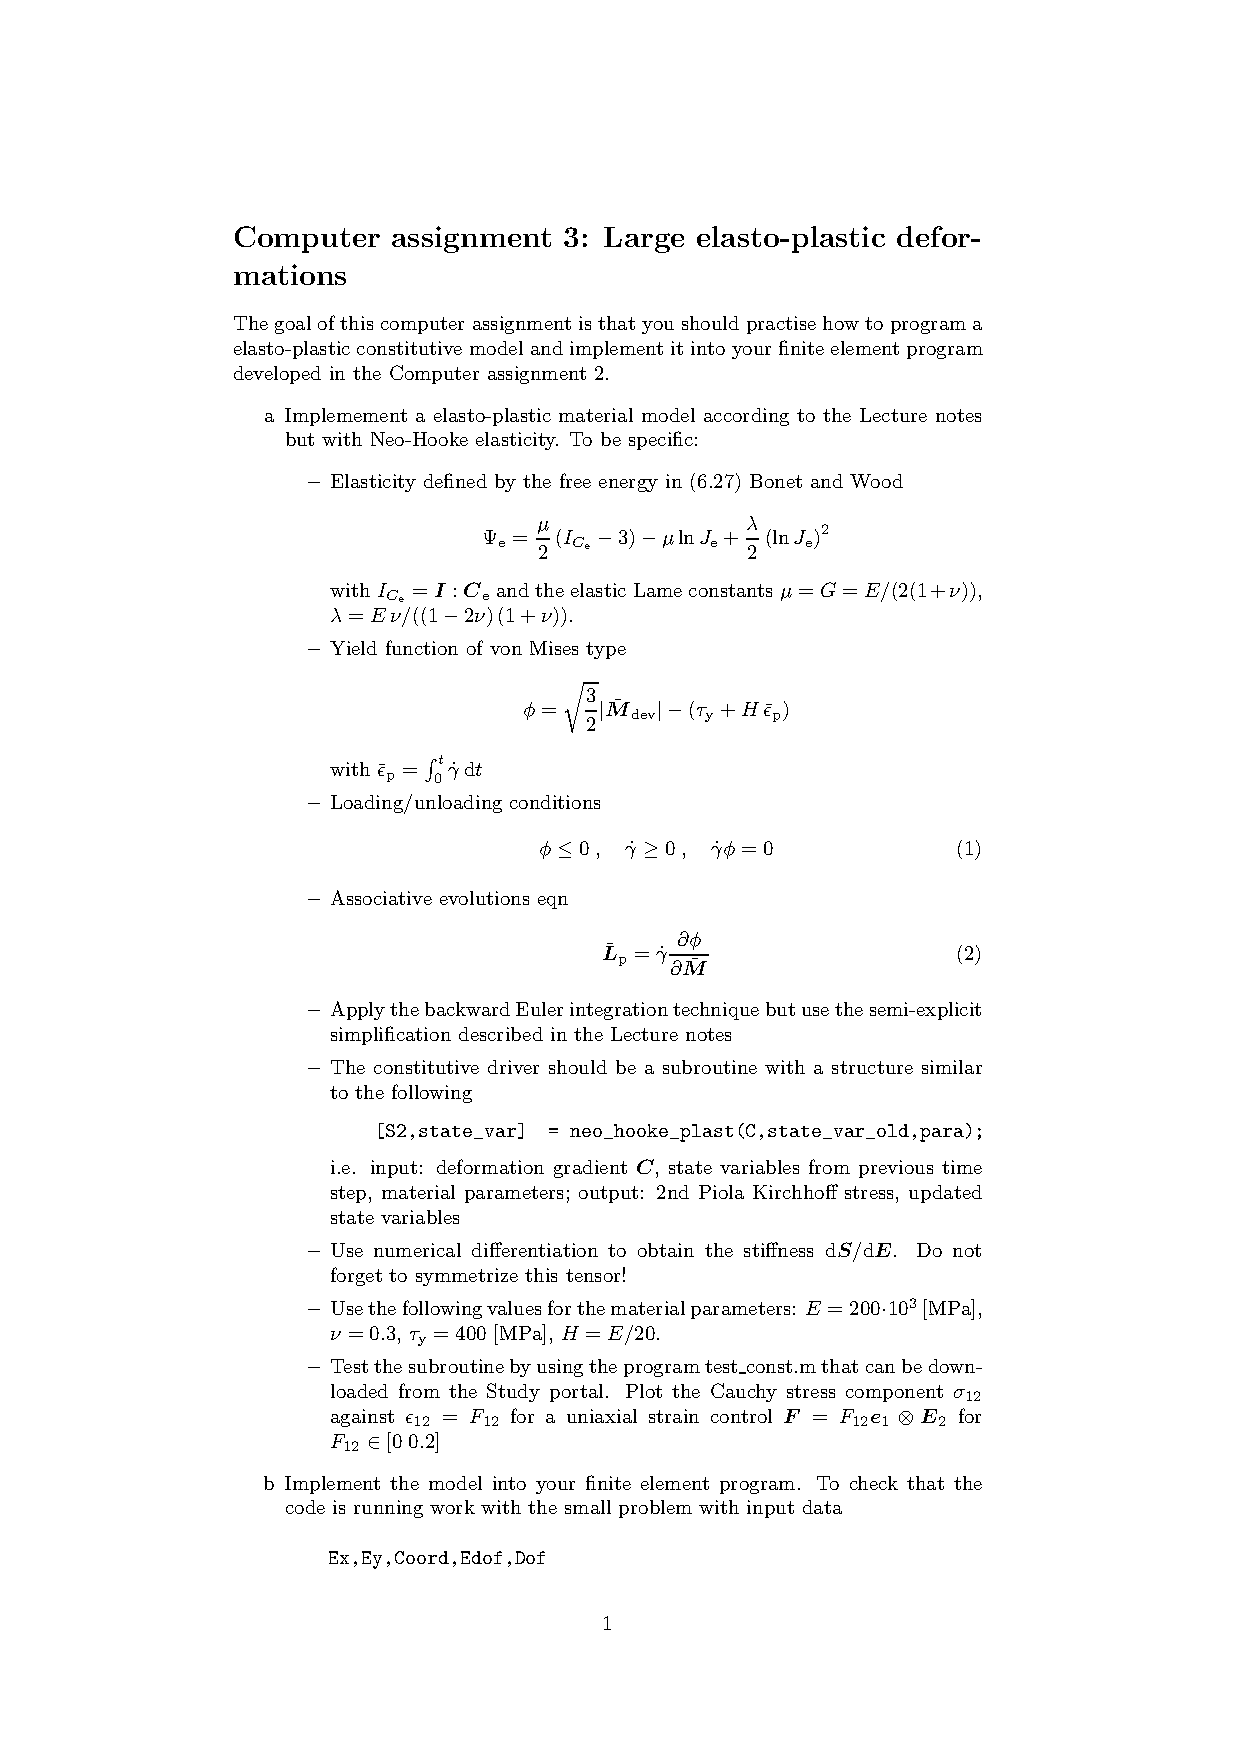
\includepdf[pages=-]{../CA3_MEkh/CA3_MEkh.pdf} % Task description.
\clearpage
\section{Task A}
\label{sec:task-a}

According to equation \eqref{eq:free-energy} in \cite{Bonet2008}, the free energy
for compressible Neo-Hookean material is defined as follows:
\begin{equation} \tag{6.27}
  \label{eq:free-energy}
  \Psi = \frac{\mu}{2} \left( I_{C_{e}} - 3 \right) - \mu \ln J_{e} +
  \frac{\lambda}{2} \left( \ln J_{e} \right)^{2}
\end{equation}
with \(I_{C_{e}} = \utilde{I} : \utilde{C}_{e} \) and the elastic Lame constants
\(\mu = G = 0.5 E / (1+\nu)\), \(\lambda = E \nu / (1 - 2\nu) / (1+\nu)\).

Yield function of von Mises type:
\begin{equation}
  \label{eq:yield_func}
  \phi = \sqrt{\frac{3}{2}} \left| \utilde{\overline{M}}_{dev} \right|- 
    \left( \tau_{y} - H \overline{\varepsilon}_{p} \right)
\end{equation}
with \(\overline{\varepsilon}_{p} = \int_{0}^{t} \dot{\gamma} \, dt\).

Mandel stress is defined as
\begin{equation}
  \label{eq:mandel}
  \utilde{\overline{M}} = \utilde{C}_{e} \cdot \widetilde{\utilde{S}}
\end{equation}
with intermediate 2nd Piola-Kirchhoff stress defined as a pull-back of the
Kirchhoff stress to the intermediate configuration as follows:
\begin{equation}
  \label{eq:PK2int}
  \widetilde{\utilde{S}} = \utilde{F}_{e}^{-1} \cdot \utilde{\tau} \cdot
  \utilde{F}_{e}^{-T} = 2 \frac{\partial \Psi}{\partial \utilde{C}_{e}}
\end{equation}
and intermediate elastic deformation tensor
\begin{equation}
  \label{eq:Cint}
  \utilde{C}_{e} = \utilde{F}_{p}^{-T} \cdot \utilde{C} \cdot \utilde{F}_{p}^{-1}
\end{equation}
and plastic part of the deformation gradient
\begin{equation}
  \label{eq:F}
  \utilde{F} = \utilde{F}_{e} \cdot \utilde{F}_{p}
\end{equation}

Let us derive expression for \(\widetilde{\utilde{S}}\):
\begin{equation}
  \label{eq:PK2intDeriv}
  \widetilde{\utilde{S}} = 2 \frac{\partial \Psi}{\partial \utilde{C}_{e}} = 
  2 \frac{\partial \Psi}{\partial I_{C_{e}}} \cdot
  \frac{\partial I_{C_{e}}}{\partial \utilde{C}_{e}} +
  2 \frac{\partial \Psi}{\partial J_{e}} \cdot
  \frac{\partial J_{e}}{\partial \utilde{C}_{e}}
\end{equation}
\begin{align}
  \frac{\partial \Psi}{\partial I_{C_{e}}} &= \frac{\mu}{2} \\
  \frac{\partial I_{C_{e}}}{\partial \utilde{C}_{e}} &= \utilde{I} \\
  \frac{\partial \Psi}{\partial J_{e}} &= - \frac{\mu}{J_{e}} + 
                                         \frac{\lambda}{J_{e}} \ln J_{e} \\
  \frac{\partial J_{e}}{\partial \utilde{C}_{e}} &= \frac{J_{e}}{2} \utilde{C}_{e}^{-1}
\end{align}
Therefore,
\begin{equation}
  \label{eq:PK2intFinal}
  \widetilde{\utilde{S}} = \mu \utilde{I} + \left( \lambda \ln J_{e} -
    \mu \right) \utilde{C}_{e}^{-1}
\end{equation}
At this point we can assess the yield function. 
The Kuhn-Tucker conditions are
\begin{equation}
  \label{eq:kuhn-tucker}
  \phi \leq 0, \quad \dot{\gamma} \geq 0, \quad \dot{\gamma} \phi = 0 
\end{equation}
The evolution equation is of associative type:
\begin{equation}
  \label{eq:evolution}
  \overline{\utilde{L}}_{p} = \dot{\gamma}
  \frac{\partial \phi}{\partial \overline{\utilde{M}}} = 
  \dot{\gamma} \sqrt{\frac{3}{2}} 
  \frac{\overline{\utilde{M}}_{dev}}{\left| \overline{\utilde{M}}_{dev} \right|} =
  \dot{\gamma} \utilde{\nu}
\end{equation}
Apply backward Euler integration:
\begin{align}
  \frac{\prescript{n+1}{}{\utilde{F}_{p} -\prescript{n}{}{\utilde{F}_{p}}}}{\Delta t}
  \prescript{n+1}{}{\utilde{F}}_{p}^{-1} &= \frac{\Delta \gamma}{\Delta t} 
                                           \prescript{n+1}{}{\utilde{\nu}} \\
  \utilde{I} - \prescript{n}{}{\utilde{F}}_{p} \cdot
  \prescript{n+1}{}{\utilde{F}}_{p}^{-1} &\approx
  \Delta \gamma \prescript{n+1}{}{\utilde{\nu}}
\end{align}
Apply semi-explicit simplification 
\(\prescript{n+1}{}{\utilde{\nu}} \approx \prescript{n}{}{\utilde{\nu}}\):
\begin{align}
  \utilde{I} - \prescript{n}{}{\utilde{F}}_{p} \cdot
  \prescript{n+1}{}{\utilde{F}}_{p}^{-1} &\approx
  \Delta \gamma \prescript{n}{}{\utilde{\nu}} \\
  \prescript{n+1}{}{\utilde{F}}_{p}^{-1} &\approx
  \prescript{n}{}{\utilde{F}}_{p}^{-1} \left( \utilde{I} -
  \Delta \gamma \prescript{n}{}{\utilde{\nu}} \right)
\end{align}
Solve the simplified local constitutive problem:
\begin{equation}
  \label{eq:local}
  \phi \left( \Delta \gamma \right) = \sqrt{\frac{3}{2}} 
  \left| \overline{\utilde{M}}_{dev} \right| - \left[ \tau_{y} - 
    H \left( \prescript{n}{}{\overline{\varepsilon}_{p}} + \Delta \gamma\right) \right]
\end{equation}
with 
\begin{equation}
  \label{eq:Mexplicit}
  \overline{\utilde{M}} = \utilde{C}_{e} \cdot \widetilde{\utilde{S}} = 
  \utilde{C}_{e} \left( \utilde{F}_{p}^{-1} \left( \Delta \gamma \right),
    \utilde{C} \right) \cdot
  \widetilde{\utilde{S}} \left( \utilde{C}_{e}
    \left( \utilde{F}_{p}^{-1} \left( \Delta \gamma \right), \utilde{C} \right)
  \right)
\end{equation}
using Newton--Raphson method:
\begin{align}
  \phi \left( \Delta \gamma_{n+1} \right) &\approx 
                                            \phi \left( \Delta \gamma_{n} \right) +
                                            \frac{d \, \phi \left( 
                                            \Delta \gamma_{n} \right)}{d \,
                                            \Delta \gamma} \blacktriangle \gamma 
                                            = 0 \\
  \blacktriangle \gamma &= - \left[ \frac{d \, \phi \left( 
                          \Delta \gamma_{n} \right)}{d \, \Delta \gamma} 
                          \right]^{-1} \cdot \phi \left( \Delta \gamma_{n} \right)\\
  \Delta \gamma_{n+1} &= \Delta \gamma_{n} + \blacktriangle \gamma
\end{align}
where the derivative of the yield function can be expanded to
\begin{equation}
  \label{eq:yield-deriv}
  \frac{d \phi}{d \gamma} = \frac{\partial \phi}{\partial \overline{\utilde{M}}} :
  \frac{\partial \overline{\utilde{M}}}{\partial \utilde{C}_{e}} :
  \frac{\partial \utilde{C}_{e}}{\partial \utilde{F}_{p}^{-1}} :
  \frac{d \utilde{F}_{p}^{-1}}{d \Delta \gamma} + 
  \frac{\partial \phi}{\partial \Delta \gamma}
\end{equation}
with \(\dfrac{\partial \phi}{\partial \Delta \gamma} = - H\) and the rest of
the derivatives given by equations (34)--(37) of \cite{Ekh2016}, in which
\begin{equation}
  \label{eq:dSdCe}
  \frac{\partial \widetilde{\utilde{S}}}{\partial \utilde{C}_{e}} = 
  \frac{\lambda}{2} \utilde{C}_{e}^{-1} \otimes \utilde{C}_{e}^{-1} +
  \left( \mu - \lambda \ln J_{e} \right) \utilde{C}_{e}^{-1} \overline{\otimes}
  \utilde{C}_{e}^{-1}
\end{equation}
Finally, compute the 2nd Piola-Kirchhoff stress
\begin{equation}
  \label{eq:PK2final}
  \utilde{S} = \utilde{F}_{p}^{-1} \cdot \widetilde{\utilde{S}} \cdot
  \utilde{F}_{p}^{-T}
\end{equation}
and the material stiffness
\begin{equation}
  \label{eq:mat-stiff}
  \uutilde{C} = 2 \frac{d \utilde{S}}{d \utilde{C}}
\end{equation}
\textit{Note: if computed numerically, \(\uutilde{C}\) must be symmetrised to get
correct element stiffness.}

The material model was implemented in Matlab and can be found in
\texttt{neo\_hooke\_plast.m} (see section \ref{app:matlab-code}).

Figure~\ref{fig:sigma12-eps12} shows the test of the constitutive driver,
where component of Cauchy stress plotted against
engineering strain for the situation of uniaxial strain control
\(\utilde{F} = F_{12} \ubar{\bm{e}}_{1} \otimes \ubar{\bm{E}}_{2}\).
\begin{figure}[th]
  \centering
  \begin{tikzpicture}
    \begin{axis}[
      width = 0.95\textwidth,
      height=\axisdefaultheight,
      tick label style={/pgf/number format/fixed},
      try min ticks=6,
      minor tick num=1,
      grid=both,
      xmin=0, xmax=0.2,
      xlabel = {\( \varepsilon_{12}\), [-]},
      ylabel = {\( \sigma_{12} \), [MPa]},
      ]
      \addplot table[skip first n=1] {data/sigma12_eps12.dat};
    \end{axis}
  \end{tikzpicture}  
  \caption{Cauchy stress component \(\sigma_{12}\) versus strain
    \(\varepsilon_{12} = F_{12} \).}
  \label{fig:sigma12-eps12}
\end{figure}


%%% Local Variables:
%%% mode: latex
%%% TeX-master: "../main"
%%% End:
 % \include uses pre- and post- \clearpage.
\section{Task B}
\label{sec:task-b}

The given boundary value problem has been solved using Matlab script
\texttt{test\_plate\_shear.m} (see section \ref{app:matlab-code}).
Figure \ref{fig:small-bvp} shows total reaction force plotted against
displacement of the top nodes and the shape of the plate before
and after the deformation.
\begin{figure}[th]
  \centering
  % Reaction force
  \begin{subfigure}[t]{\textwidth}
    \begin{tikzpicture}
      \begin{axis}[
        width = 0.95\textwidth,
        height=\axisdefaultheight,
        tick label style={/pgf/number format/fixed},
        try min ticks=6,
        minor tick num=1,
        grid=both,
        xlabel = {\(u_{x}\), [mm]},
        ylabel = {Reaction force, [N]},
        xmin=0, xmax=0.1, ymax=550
        ]
        \addplot table[skip first n=1] {data/force_displacement.dat};
      \end{axis}
    \end{tikzpicture}
    \caption{}
  \end{subfigure}

  % Geometry
  \begin{subfigure}[t]{\textwidth}
    \begin{tikzpicture}
      \begin{axis}[
        width = 0.95\textwidth,
        try min ticks=6,
        enlargelimits=false,
        axis equal image,
        axis on top,
        xlabel={\(x\), [mm]},
        ylabel={\(y\), [mm]}
        ]
        \addplot graphics[xmin=-0.9945,xmax=-0.1363,
                          ymin=-0.3132,ymax=0.3352] {small_mesh};
      \end{axis}
    \end{tikzpicture}  
    \caption{}
  \end{subfigure}
  \caption{(a) Reaction force versus displacement and (b) deformed mesh.}
  \label{fig:small-bvp}
\end{figure}


%%% Local Variables:
%%% mode: latex
%%% TeX-master: "../main"
%%% End:
 
\section{Task C}
\label{sec:task-c}

The second boundary value problem has been solved using Matlab script
\texttt{forming\_process.m} (see section \ref{app:matlab-code}).
Figure \ref{fig:forming-bvp} shows total reaction force plotted against
displacement of the top nodes and the shape of the plate before
and after the deformation.
\begin{figure}[th]
  \centering
  % Reaction force
  \begin{subfigure}[t]{\textwidth}
    \begin{tikzpicture}
      \begin{axis}[
        width = 0.95\textwidth,
        height=\axisdefaultheight,
        tick label style={/pgf/number format/fixed},
        try min ticks=6,
        minor tick num=1,
        grid=both,
        xlabel = {\(u_{x}\), [mm]},
        ylabel = {Reaction force, [N]},
        xmin=0, xmax=5, ymax=1.6e4
        ]
        \addplot table[skip first n=1] {data/force_displacement_forming.dat};
      \end{axis}
    \end{tikzpicture}
    \caption{}
  \end{subfigure}

  % Geometry
  \begin{subfigure}[t]{\textwidth}
    \begin{tikzpicture}
      \begin{axis}[
        width = 0.95\textwidth,
        try min ticks=6,
        enlargelimits=false,
        axis equal image,
        axis on top,
        xlabel={\(x\), [mm]},
        ylabel={\(y\), [mm]}
        ]
        \addplot graphics[xmin=0,xmax=24.66,
                          ymin=0,ymax=20] {plate_with_hole_mesh};
      \end{axis}
    \end{tikzpicture}  
    \caption{}
  \end{subfigure}
  \caption{(a) Reaction force versus displacement and (b) deformed mesh.}
  \label{fig:forming-bvp}
\end{figure}


%%% Local Variables:
%%% mode: latex
%%% TeX-master: "../main"
%%% End:
 
\section{Task D}
\label{sec:task-d}

The logarithmic strain model from chapter 5 \cite{Ekh2016} was implemented
in Matlab function \texttt{neo\_hooke\_plast\_log\_strain.m} (see 
section \ref{app:matlab-code}) and applied to solve the same boundary 
value problem as in section \ref{sec:task-c}.
Figure \ref{fig:forming-bvp-log-strain} compares the total reaction force
plotted against displacement of the top nodes for the two models.
The two models yield virtually the same graphs.
\begin{figure}[th]
  \centering
  % Reaction force
    \begin{tikzpicture}
      \begin{axis}[
        width = 0.95\textwidth,
        height=\axisdefaultheight,
        tick label style={/pgf/number format/fixed},
        try min ticks=6,
        minor tick num=1,
        grid=both,
        legend style={at={(0.5,0)},
          anchor=south},
        xlabel = {\(u_{x}\), [mm]},
        ylabel = {Reaction force, [N]},
        xmin=0, xmax=5,
        ]
        \addplot[mark=none, blue] table[skip first n=1]
        {data/force_displacement_forming.dat};
        \addlegendentry{Neo-Hooke}
        \addplot[mark=none, red, dashed] table[skip first n=1]
        {data/force_displacement_log_strain.dat};
        \addlegendentry{Neo-Hooke, log strain}
      \end{axis}
    \end{tikzpicture}
    \caption{Reaction force versus displacement.}
  \label{fig:forming-bvp-log-strain}
\end{figure}


%%% Local Variables:
%%% mode: latex
%%% TeX-master: "../main"
%%% End:
 
\section{Matlab code}
\label{app:matlab-code}

The Matlab code can be found in the Git repository on
\href{https://github.com/iamrosk/large_elast_plast_deform}{Github}.

%%% Local Variables:
%%% mode: latex
%%% TeX-master: "../main"
%%% End:


\bibliographystyle{abbrv}
\bibliography{references}

\end{document}

%%% Local Variables:
%%% mode: latex
%%% TeX-master: t
%%% End:
